\chapter{Theorie}
\label{cha:Theorie}
\section{Mikrowellen}
\label{sec:mikrowellen}
In diesem Versuch werden lediglich Mikrowellen betrachtet. Das heißt ein Frequenzbereich von $\qty{1}{\giga\hertz}$-$\qty{300}{\giga\hertz}$ beziehungsweise eine Wellenlänge von 
$\sim \qty{33.3}{\milli\metre}$. Dieser Frequenzbereich ist sehr interessant, da Mikrowellen in der Atmosphäre nicht stark reflektiert oder absorbiert werden.
\subsection{Stehende Wellen}
\label{subsec:stehende_Welle}
Generell werden elektromagnetische Wellen durch die Maxwell Gleichungen beschrieben. In diesem Experiment werden allerdings Wellen in einem Hohlleiter betrachtet, welcher im Abschnitt 
\ref{subsec:hohlleiter} noch beschrieben wird. Daher genügt es die einfachste Form einer ebenen Welle zu betrachten.
\begin{equation*}
              A(x,t) = A_0sin(kx\pm\omega t)
\end{equation*}
In dieser Gleichung ist $A_0$ die Amplitude, $k$ die Wellenzahl, $\omega$ die Kreisfrequenz. Das Vorzeichen gibt die Laufrichtung der Welle an. Für einen Hohlleiter ist es ebenfalls 
genügend ein eindimensionales Problem zu betrachten. Um eine stehende Welle zu erzeugen werden nun allerdings mindestens zwei ebene Wellen benötigt, da dies ein Interferenzeffekt ist.
Das ebene Wellen die Kohärenzbedingungen erfüllen wird an dieser Stelle nicht näher diskutiert, da das Hauptaugenmerk später auf dem Klystron liegen soll. Wir betrachten zunächst eine
einfache ebene Welle. Diese kann nun an einem Medium totalreflektiert werden, also die volle Amplitude bleibt erhalten. Nun existiert eine rechtslaufende Welle vor der Reflexion und
eine linkslaufende Welle nach der Reflexion. 

\begin{equation*}
              A(x,t) = A_0\sin(kx - \omega t) + A_0\sin(kx + \omega t)
\end{equation*}

Dieser Term kann in Gleichung \ref{eqn:steh_welle} umgeschrieben werden.

\begin{equation}
              \label{eqn:steh_welle}
              A(x,t) = 2A_0\sin(kx)\cos(\omega t)
\end{equation}

In dieser Gleichung erkennt man, dass es räumlich feste Nullstellen gibt und die Welle nur noch zwischen diesen schwingt.

\subsection{Stehwellenverhältnis}
\label{subsec:Stehwellenverhaeltnis}
Gleichung \ref{eqn:steh_welle} gilt lediglich für totale Reflexion. Aber im Anwendungsfall tritt so etwas nie auf, stattdessen treten weitere Mischterme in der überlagerten Welle auf.
Dies geschieht nicht nur aufgrund von Transmissionseffekten, sondern auch durch Unstetigkeiten im Medium. Aufgrund dieser Mischterme entstehen keine Nullstellen, sonder
lediglich Minima und Maxima der Amplitude. Das Verhältnis von Maxima und Minima wird Stehwellenverhältnis genannt.

\begin{equation}
              \label{eqn:SWR}
              S = \frac{E_\mathrm{max}}{E_\mathrm{min}}, S\in[1,\infty]
\end{equation}

Es beschreibt die Welligkeit der überlagerten Stehwelle. Je größer
das Stehwellenverhältnis, desto gößer ist das Maximum und oder kleiner ist das Minimum. Bei einer perfekten stehenden Welle divergiert das Stehwellenverhältnis. Eine mögliche
Stehwelle wird in Abbildung \ref{fig:stehwelle} dargestellt.

\begin{figure}
              \centering
              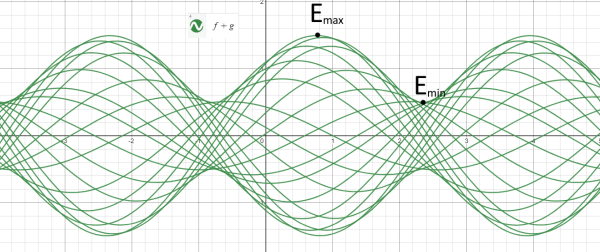
\includegraphics[width = .9\textwidth]{content/stehwelle.PNG}
              \caption{In dieser Abbildung wird eine stehende Welle mit festem Stehwellenverhältnis dargestellt.}
              \label{fig:stehwelle}
\end{figure}

Für die in der Durchführung beschriebene $\qty{3}{\decibel}$-Methode in \autoref{subsec:3db_methode} kann das Stehwellenverhältnis durch 
\begin{equation}
              \label{eqn:S_3dB}
              S = \sqrt{1+\frac{1}{\sin^2\left(\frac{\pi(x_\mathrm{links}-x_\mathrm{rechts})}{\lambda_\mathrm{H}}\right)}}
\end{equation}
berechnet werden. Wenn $\lambda_H >> x_\mathrm{links}-x_\mathrm{rechts}$ kann man das SWR (Stehwellenverhältnis) durch 
\begin{equation}
              \label{eqn:S_3dB_easy}
              S = \frac{\lambda_H}{\pi(x_\mathrm{links}-x_\mathrm{rechts})}
\end{equation}
genähert werden aufgrund der Kleinwinkelnäherung.

Bei der Abschwächer-Methode, welche in \autoref{subsec:abschwächer} beschrieben wird, kann das SWR durch 
\begin{equation}
              \label{eqn:S_abschwaecher}
              S = 10^\frac{A_2-A1}{\qty{20}{\decibel}}
\end{equation}
beschrieben werden.
\subsection{Welle im Hohlleiter}
\label{subsec:hohlleiter}
Ein Hohlleiter ist zunächst erstmal ein hohles, das heißt eine innen nicht festes, Objekt. Dieses besteht aus einer leitenden Oberfläche, also meistens aus Metallen. Es dient der 
"Leitung" von Wellen und wird verwendet, da der Leistungstransfer im Frequenzbereich von $\qty{1}{\giga\hertz}$ bis $\qty{1500}{\giga\hertz}$ verlustärmer ist. In diesem Experiment
wird ein rechteckiger Hohlleiter, welcher mit Umgebungsluft gefüllt ist verwendet. Eine Skizze wird in Abbildung \ref{fig:hohlleiter} gezeigt.

\begin{figure}
              \centering
              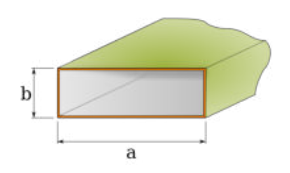
\includegraphics{content/hohlleiter.PNG}
              \caption{In dieser Abbildung werden schematisch die Seitenlängen eines Hohlleiters dargestellt.}
              \label{fig:hohlleiter}
\end{figure}

Nun ist es wichtig zwischen Hohlraumresonatoren und Hohlleitern zu unterscheiden, da diese 
prinzipiell sehr ähnlich sind. Ein Hohlraumresonator ist ein geschlossenes innen hohles Objekt. Das bedeutet eine Welle in diesem Hohlraumresonator kann in alle kartesischen Richtungen
an der Innenfläche reflektiert werden. Im Hohlleiter dagegen verhält es sich wie in einem Kabel. Er ist aufgebaut wie ein langes rechteckiges Rohr mit den Seitenlängen $a$ und $b$. Die 
Welle in einem Hohlleiter kann daher nur in eine Richtung propagieren. In den anderen beiden Raumrichtungen wird sie reflektiert. Dabei entsteht eine stehende Welle orthogonal zur 
Öffnung, welche aber in Richtung der Öffnung verläuft. Aufgrund der ähnlichkeit zum Hohlraumresonator existiert auch hier eine untere Grenzfrequenz, ab welcher stehende Welle 
in einem rechteckigen Hohlleiter entstehen können. Dazu korrespondiert die kritische Wellenlänge 

\begin{equation}
              \label{eqn:lambda_g}
              \lambda_g = \frac{2}{\sqrt{\frac{m}{a}^2+\frac{n}{b}^2}}%n ergänzen
\end{equation}

Daber sind $a$ und $b$ die Seitenlängen des in Abbildung \ref{fig:hohlleiter} dargestellten Hohlleiters. Diese Grenzwellenlänge gilt für $\textbf{TEM}_m$, wobei der index $n$ die Zahl 
der Mode ist. Das heißt eine Mode wird durch $m,n$ charakterisiert. Unterhalb dieser Wellenlänge kann die Wellenlänge im Hohlleiter durch die Wellenlänge im freien Raum durch 
\begin{equation}
              \label{eqn:lambda_g}
              \lambda_0 = \frac{\lambda_g}{1-\left(\frac{\lambda_0}{\lambda_c}\right)^2}
\end{equation}
berechnet werden. 
Für eine $\mathrm{TE}_{10}$ kann die Frequenz $f = \sfrac{c}{\lambda_0}$ durch 
\begin{equation}
              \label{eqn:TE01}
              f = c\sqrt{\left(\frac{1}{\lambda_g}\right)^2+\left(\frac{1}{2a}\right)^2}
\end{equation}


\section{Reflexklystron}
\label{sec:reflexklystron}
Ein Reflexklystron wird zur Erzeugung von Mikrowellen verwendet. Dabei kann man diese aus dem Reflexklystron auskoppeln um diese dann auf einem Hohlleiter propagieren zu lassen oder 
für die jeweilige Anwendung nutzen. Das Reflexklystron ist dabei eine Entwicklungsstufe des klassischen Klystrons. Die Funktionsweise ist änhlich jedoch unterscheidet sich der Aubau.
\subsection{Aufbau eines Reflexklystron}
\label{subsec:aufbau_klystron}
Eine Skizze des Aufbaus wird in Abbildung \ref{fig:reflexklystron} dargestellt. Es besteht aus einer Glühkathode und einer Refloktoranode und zwei Hohlraumresonatorkammern. Hinter 
der Kathode liegt ein Beschleunigungsgitter an. Danach treffen die beschleunigten Elektronen auf den Hohlraumresonator. Nachdem dieser durchlaufen wurde, treffen die Elektronen auf 
den Reflektor anhand desse diese umgekhert werden und erneut auf den Hohlraumresonator treffen. Dies ist ein fortlaufender Prozess. Eine Hohlraumkammer dient dabei als wirklicher 
Hohlraumresonator und die andere als Auskopplungskammer.
\begin{figure}
              \centering
              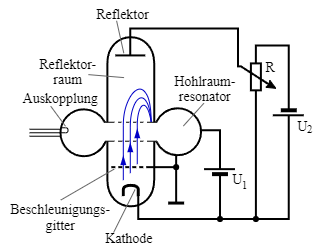
\includegraphics{content/reflexklystron.PNG}
              \caption{In dieser Abbildung wird der grundlegende Aufbau eines Reflexklystrons dargestellt.}
              \label{fig:reflexklystron}
\end{figure}
\subsection{Funktionsweise des Reflexklystrons}
\label{subsec:funktion}
Wie bereits erwähnt durchläuft der Elektronenstrahl zunächst den mit einer stehenden Welle gespeisten Hohlraumresonator. Die Elektronen werden dabei Geschwindigkeitsmoduliert.
Das geschieht jenach lokaler Feldstärke der stehenden Welle. Da die Elektronen also unterschiedlich stark in ihrer Geschwindigkeit moduliert werden, ist das gleichbedeutent mit einer
Dichtemodulation des Elektronenstrahls. Dies nennt man \textit{bunching}. Dieser dichtemodulierte Elektronenstrahl trifft nun auf den Reflektor und wir umgekhert. Nun durchläuft er 
erneut de stehende Welle. Nun können zwei Effekte auftreten. Jenachdem, ob der \textit{gebunchte} Elektronenstrahl nun auf ein Maximum oder Minimum trifft kann ein dämpfender oder 
resonanter Effekt auftreten. Trifft der \textit{gebunchte} Strahl mit einem Maximum an Elektronen nun auf ein Maximum des $\vec{E}$-Feldes, also auf ein positives Feld, so wird 
Energie in die Stehwelle eingekoppelt. Es tritt also eine resonante Wechselwirkung auf. Andernfalls kann ein Maximum des \textit{gebunchte} Strahls auf ein minimales Feld, also 
ein negatives Feld, treffen. Dabei nimmt der Strahl Energie der Welle auf und dämpft diese damit. Es tritt also ein dämpfender Effekt auf. Das Auftreten eines Effektes hängt von der 
technischen Umsetzung, beziehungsweise den technischen Parametern ab. Eine einfache Methode der Einstellung eines Falles ist die Änderung der Spannung am Reflektor, aber es können 
ebenfalls die Höhe des Reflektors oder andere geometrische Eigenschaften verändert werden. Der Bunching-Prozess wird anschaulich an Abbildung \ref{fig:bunching} dargestellt.

\begin{figure}
              \centering
              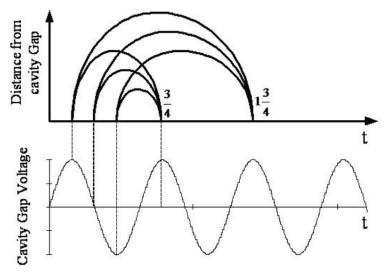
\includegraphics{content/bunching.PNG}
              \caption{In dieser Abbildung wird der bunching Prozess dargestellt. Dies gilt für Parameter welche einen optimal Energieübertrag erzeugen. Dabei ist $t$ in Einheiten von 
              $T_0$, der Periodendauer der Hohlraumresonatorfrequenz, angegeben.}
              \label{fig:bunching}
\end{figure}

\subsection{Moden im Klystron}
\label{subsec:moden}
Für einen optimal Energieübertrag muss daher die geometrische Bedingung $t = T_0\left(n+\sfrac{3}{4}\right)$ erfüllt sein. Mit dieser Bedingung folgen Moden, welche in Abbildung 
\ref{fig:moden} dargestellt werden. 

\begin{figure}
              \centering
              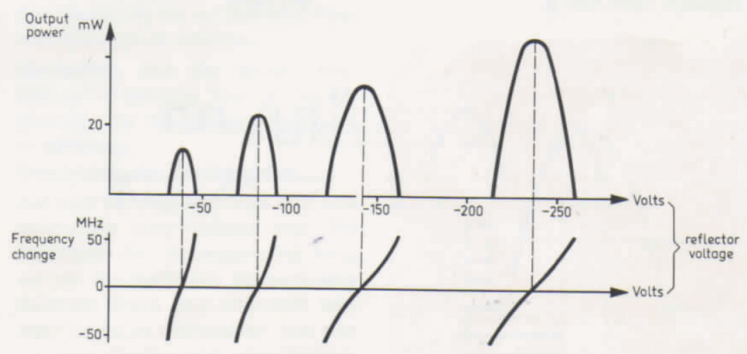
\includegraphics[width = .9\textwidth]{content/moden.PNG}
              \caption{In dieser Abbildung werden die Moden des Rexlexklystrons in Abhängigkeit der Reflektorspannung dargestellt.}
              \label{fig:moden}
\end{figure}

Dabei wird in dem oberen Graphen deutlich, dass der Energieübertrag parabelförmig um ein Maximum stattfindet. Außerdem ist zu beachten, dass die unterschiedlichen Energieüberträge 
ebenfalls etwas die Frequenz der Welle verändern. Deshalb wird ein Frequenzmesser eingebaut, welcher einen kleinen Teil der Energie auskoppelt, um so die Frequenz messen zu können.
Der Frequenzmesser ist vor der Sonde plaziert, daher ist aufgrund der Entkopplung ein kleiner Spannungseinbruch sichtbar. Dies ermöglicht überhaupt erst die Frequenzmessung.

\section{Einwegrichter}
\label{sec:einwegrichter}

Zuletzt wird nun der Einwegrichter eklärt. Dieser wird innerhalb des Hohlleiters verwendet, damit die Strahlung nur in eine Richtung propagieren kann. Der Einwegrichter besteht aus 
einem Permanentmagneten. Durch den Farady-Effekt lenkt dieser die Strahlung ab. Beiden Strahlenrichtungen werden aber betragsmäßg gleich abgelenkt. Daher wird zusätzlich ein 
Strahlen-Tor verwendet um eine Absorption in eine Richtung zu erhlten und Transmission in die entgegengesetzte.

